\newpage

%%%%% ---------- the background picture ---------- %%%%%
%% to change it modify the macro \BackgroundPicture
\ClearShipoutPicture
\AddToShipoutPicture{\BackgroundPicture}

\noindent % to have the picture right in the center
\begin{tikzpicture}
  \initializesizeandshifts
  \setxshift{21.5}
  % \setyshift{2}


  %% the title block, #1 - shift, the default value is (0,0), #2 - width, #3 - scale
  %% the alias of the title block is `title', so we can refer to its boundaries later
  \ifthenelse{\equal{\template}{1}}{ 
    \titleblock{47}{1}
  }{
    \titleblock{49}{1.5}
  }

  %% a logo can be added to the title block
  %% #1 - anchor relative to the title block, #2 - shift, #3 - width, #3 - file name
   \ifthenelse{\equal{\template}{2}}{ 
     \addlogo[south west]{(-5,0)}{11cm}{./figures/CAS}
   }{
     \addlogo[south west]{(-15,-1)}{11cm}{./figures/CAS-dark}
   }


%%%%%%%%%% ------------------------------------------ %%%%%%%%%%
\blocknodew[($(currenty)-(4.5,0)$)]{32}{选题背景和意义} %
{\innerblock{研究背景}{
\qquad 人体组织主要由胞外基质(extracellular matrix), 胞外基质中的细胞, 及作用于胞外基质和细胞间的间质流体(interstitial fluid)组成. 三者相互作用共同决定了肿瘤的发生和发展:
\begin{itemize}
\item 间质流在肿瘤生长和迁移中起到了重要作用. 肿瘤生长时, 它们促进肿瘤本身和周围组织内部的新血管生成. 在肿瘤迁移过程中它们提供力学刺激来引导肿瘤细胞的迁移.
\item 胞外基质直接影响着间质流动. 细胞外基质是一个复杂的大分子网络, 其刚度, 孔隙率, 空间排布和取向等特性直接影响细胞的行为及间质流动.
\item 细胞的行为和力学性能改变会反过来影响胞外基质的代谢和刚度以及间质流体的流动.
\end{itemize}
因此, \textcolor{blue}{认识胞外基质, 间质流及肿瘤细胞的力学特征和相互作用机理对于研究肿瘤发展及肿瘤细胞生物学行为具有重要意义.}
}
\vspace{-15pt}

\innerblock{研究意义}{
\qquad 本文旨在建立一套研究介观尺度多相生物流的数值模拟方法体系, 对胞外基质中的间质液流动特性进行有效, 可靠的分析和预测, 探索间质液, 细胞, 胞外基质三者的相互作用和运动机理, 理解间质流和胞外基质对肿瘤细胞生长和迁移的影响. 为肿瘤的预防, 诊断, 分析及治疗等领域的需求服务. 同时也为相关生物微型器件的设计提供依据.
}
\vspace{-30pt}
}


%%%%%%%%%% ------------------------------------------ %%%%%%%%%%
\blocknodew[($(currenty)-(0,0)$)]{32}{研究内容和研究目标} 
{ 
\qquad 本文基于耗散粒子动力学, 拟研究胞外基质, 间质液流动及细胞三者间的力学相互作用和运动机理. 该研究细分为如下阶段内容和目标:
\begin{itemize}
\item\textcolor{blue}{不同性质的流体的模拟}: 调整改进DPD的各参数和权函数, 引入新型作用势和多体DPD等模型, 以获得对不同性质(如不同粘性, 不同亲疏性等)流体的模拟.
\item\textcolor{blue}{含有刚体的流动的模拟}: 引入刚体模型研究不同孔隙率和排列方式的圆柱阵列对流体流动, 及阵列中的圆球受力的的影响, 以此初步模拟细胞外基质对细胞受间质流体作用力的影响.
\item\textcolor{blue}{高分子动力学特性研究}: 引入珠簧链模型(如WLC模型), 来模拟含有高分子的流动. 探求不同密度和长度的高分子链运动和迁移等特征. 为构建弹性细胞外基质和细胞模型作准备.
\item\textcolor{blue}{细胞模型的构建和模拟}: 用珠簧链模型, 并引入二面角等作用势来模拟细胞膜. 应用于血红细胞, 并扩展到其它细胞的模拟, 以便更真实的模拟间质流动中的细胞.
\item\textcolor{blue}{间质流动的构建和模拟}: 用珠簧链构造胞外基质和细胞, 简单DPD粒子模拟间质流体. 结合高性能计算, 模拟并研究胞外基质, 间质液流动及细胞三者间的力学相互作用和运动机理.
\end{itemize}
}

  


  %%%%%%%%%%%%% NEW COLUMN %%%%%%%%%%%%%%% 
  \startsecondcolumn 


  \blocknodew[($(currenty)-(4.5,0)$)]{51}{国内外相关研究的主要进展} %
  { 
\begin{minipage}{0.5\linewidth}
\coloredbox{colorthree!50!}{
\qquad 在实验观察方面, 由于肿瘤内部细胞的拥挤, 向外的生长应力以及外围的致密包裹使肿瘤组织的整体刚度高于周围正常组织. 目前, 广泛应用于诊断实体肿瘤弹性成像技术的准确率和分辨率, 还无法准确区分肿瘤细胞与周围间质的力学差异.
\vspace{27pt}

\qquad 在实验模拟方面, 为了模拟胞外基质和间质液流动对肿瘤细胞的影响, 细胞被植入到胶原蛋白基质之中, 然后给液体环境施加压力. 这种压力导致细胞周围的液体流动, 从而模拟生长中肿瘤的体内环境. 这允许科学家们在更加接近于生理环境的培养系统中研究和观测生长中肿瘤的微环境, 更好地理解细胞外液流动和胞外基质对肿瘤产生的影响.
}
\end{minipage}
\begin{minipage}{0.005\linewidth}
  {~}
\end{minipage}
\begin{minipage}{0.49\linewidth}
\coloredbox{colorthree!50!}{
\vspace{-7pt}
\begin{tikzfigure}[正常组织和肿瘤组织]
\begin{tikzpicture}
\node at (0,0) {\includegraphics[width=0.95\textwidth]{./figures/TumorTissue.pdf}};
\node[right] at (-10.5,-12.9) {\small Normal Tissue};
\node[right] at (3,-14) {\small Tumor Tissue};
\end{tikzpicture}
\end{tikzfigure}
}
\end{minipage}

\vspace{10pt}

\begin{minipage}{0.5\linewidth}
\coloredbox{colorthree!50!}{
\vspace{5pt}
~~~~在数值模拟方面, 生物流体的复杂性和流变特性的尺度效应等因素都给计算模型带来了很大的挑战. 
\begin{itemize}
\item 基于宏观连续力学的数值模拟方法不再适用于介观尺度多相生物流体.
\item 由于计算能力的限制, 经典分子动力学方法一般局限在纳米和纳秒量级.
\item \textcolor{blue}{介观尺度模拟方法是模拟介观尺度生物流体流动问题的合理选择}.
\end{itemize}
\vspace{8pt}
}
\end{minipage}
\begin{minipage}{0.005\linewidth}
~
\end{minipage}
\begin{minipage}{0.49\linewidth}
\coloredbox{colorthree!50!}{
\begin{tikzfigure}[不同尺度的方法]
%\begin{tikzpicture}
%\node at (0,0) {\includegraphics[width=\textwidth]{./figures/spatiotemporal.pdf}};
%\end{tikzpicture}
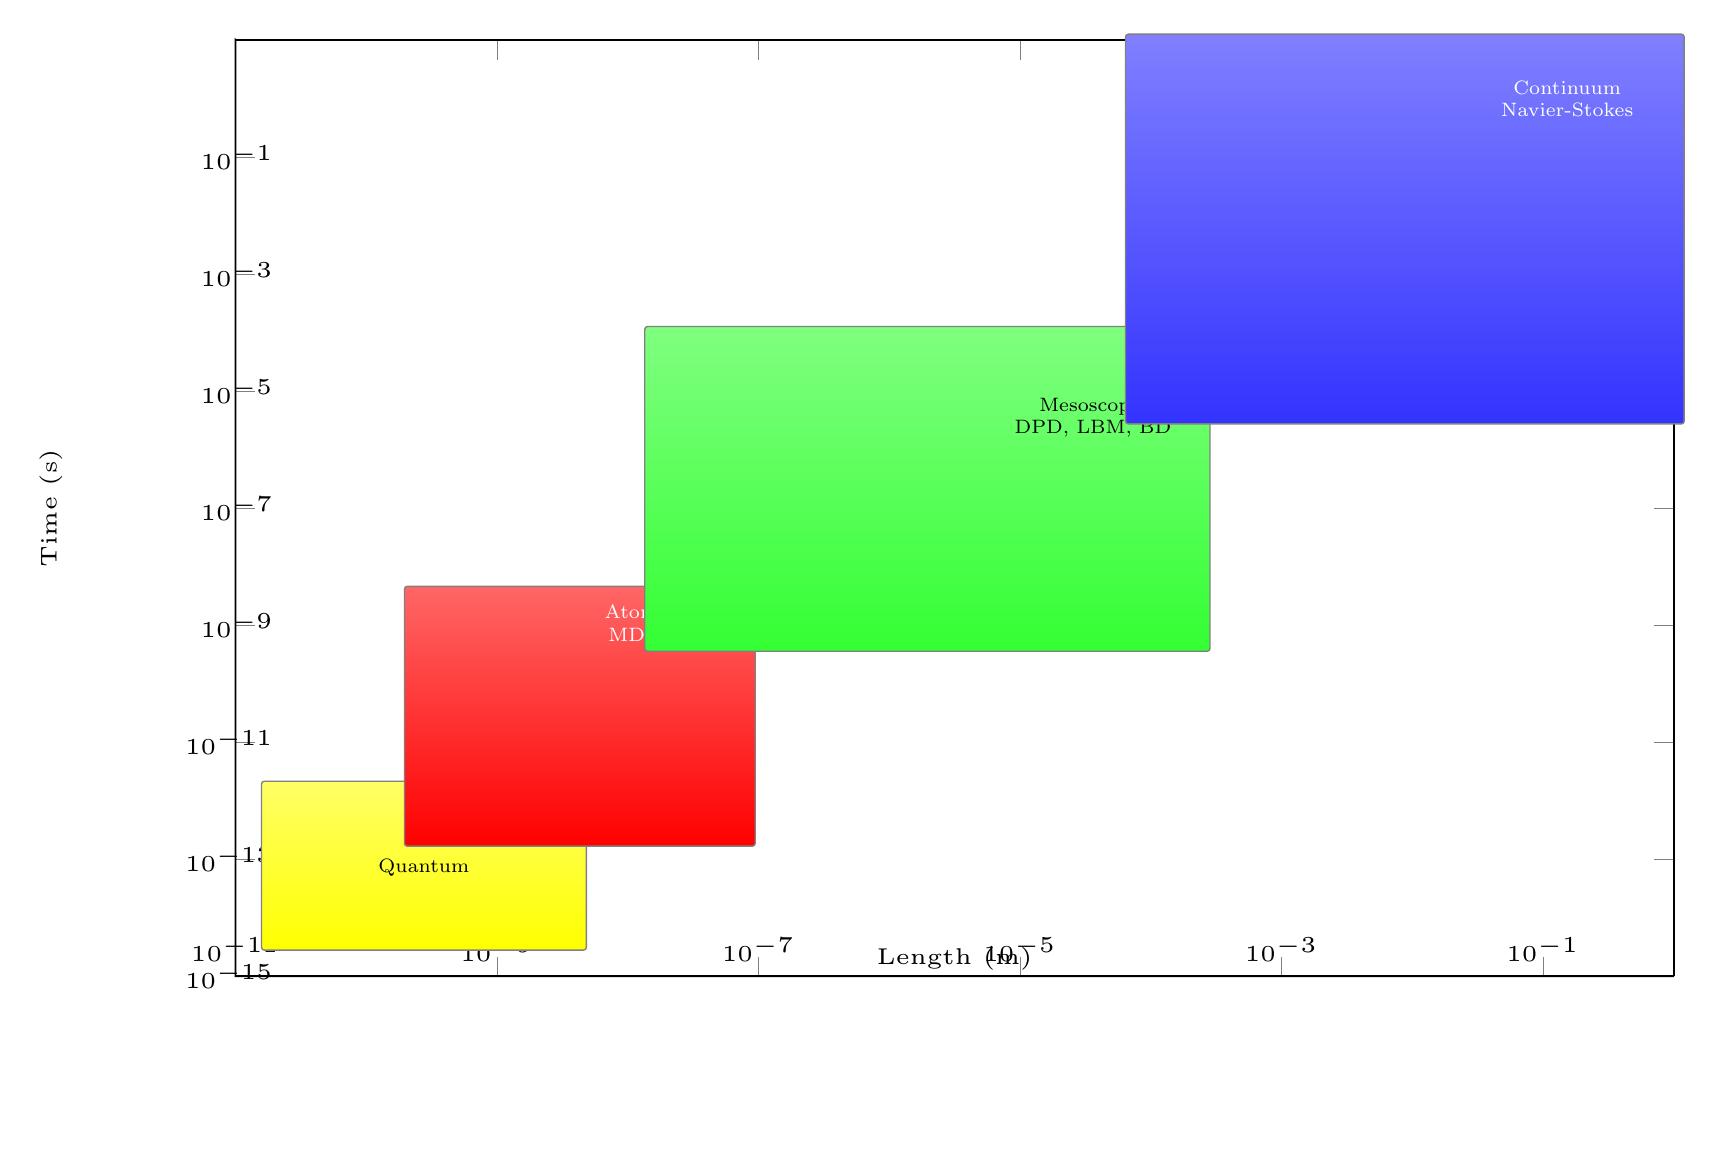
\begin{tikzpicture}[rounded corners=0em,decoration={random steps,segment length=10em,amplitude=0},scale=1.65, clip=true,line width=0.05em]
\clip(-1.6,-1.15) rectangle (11.2,7.3);
%\draw(-1.6,-1.15) rectangle (11.2,7.3);
\begin{loglogaxis}[xmin=1e-11, xmax=1.0, ymin=1e-15, ymax=10, width=360pt, height=250pt,
xlabel={Length (m)},ylabel={Time (s)},
legend style={cells={anchor=west},font=\tiny},
              tick label style={font=\tiny},
              ytick={1e-15,1e-13,1e-11,1e-9,1e-7,1e-5,1e-3,1e-1},
              xtick={1e-11,1e-9,1e-7,1e-5,1e-3,1e-1},
              label style={font=\tiny},
              ylabel style={yshift=20pt},
              xlabel style={yshift=10pt},
              xticklabel style={yshift=12pt},
              yticklabel style={xshift=12pt},clip=true
]
\end{loglogaxis}
\begin{scope}[rounded corners=0.1em]
\draw[top color=yellow!60, bottom color=yellow!100,draw=gray] (0.2,0.2)rectangle (2.7,1.5) node[black,midway,above=-0.75em,font=\scriptsize]{Quantum};

\draw[top color=yellow!60,top color=red!60, bottom color=red!100,draw=gray] (1.3,1)rectangle (4,3);
\node[font=\scriptsize,text width=4em,text centered] at (3.2,2.7){\textcolor{white}{Atomistic MD, MC}};

\draw[top color=yellow!60,top color=green!50, bottom color=green!80,draw=gray] (3.15,2.5)rectangle (7.5,5);
\node[font=\scriptsize,text width=8em,text centered] at (6.6,4.3){Mesoscopic DPD, LBM, BD};

\draw[top color=yellow!60,top color=blue!50, bottom color=blue!80,draw=gray] (6.85,4.25)rectangle (11.15,7.25);
\node[font=\scriptsize,text width=8em,text centered,white] at (10.25,6.75){Continuum Navier-Stokes};




%\node[rectangle,top color=red!60, bottom color=red!100,draw=gray,text width=2.8em,font=\scriptsize, , text height=0.8em, text centered] at (2.7,2.8){\textcolor{white}{Atomistic MD, MC}};
%\node[rectangle,top color=green!60, bottom color=green!100,draw=gray,text width=4.5em,font=\scriptsize, text height=1.4em, text centered] at (5.5,4.7){Mesoscopic DPD,LBM,BD};
%\node[rectangle,top color=blue!50, bottom color=blue!70,draw=gray,text width=8em,font=\scriptsize, text height=2em, text centered,inner sep=0.2em, inner ysep=0.5em] at (8.725,7){\textcolor{white}{Continuum Navier-Stokes}};
\end{scope}
\end{tikzpicture}

\end{tikzfigure}
}
\end{minipage}
\vspace{8pt}

}

  
\blocknodew[($(currenty)-(0,0)$)]{51}{总体研究方案} %
{

\begin{minipage}{0.6\linewidth}
\coloredbox{colorthree!50!}{
\begin{tikzfigure}[技术路线图]
\tikzstyle{decision} = [diamond, aspect=2, draw=gray,left color=blue!30, right color=red!30, 
    text width=3em, text badly centered, inner sep=0pt,rounded corners=1pt]
\tikzstyle{block} = [rectangle, draw=gray, top color=black!10, bottom color=black!30,
    text width=4em, inner sep=8pt, text centered, rounded corners, minimum height=2.1em, node distance=7cm]
\tikzstyle{blockone} = [rectangle, draw=gray, top color=blue!10, bottom color=blue!30,
    text width=4em, inner sep=8pt, text centered, rounded corners, minimum height=2.1em, node distance=7cm]
\tikzstyle{blocktwo} = [rectangle, draw=gray, top color=red!10, bottom color=red!30,
    text width=4em, inner sep=8pt, text centered, rounded corners, minimum height=2.1em, node distance=7cm]
\tikzstyle{line} = [draw,black!80]
\tikzstyle{arrow} = [draw,->, >=stealth',black!80]
\tikzstyle{cloud} = [draw, ellipse,fill=red!20, node distance=7cm,
    minimum height=2em]
{\scriptsize
\begin{tikzpicture}[x=1.8cm,y=2.5cm, node distance = 6cm, line width=0.075em]
 \clip (-1.1,-3.5) rectangle (14.6,2.9);
 %\draw (-1.1,-3.5) rectangle (14.6,2.9);
 \node[block,top color=blue!50, bottom color=blue!60] (START)  at (0, 0)  {\textcolor{white}{研究内容}};
 \node[block,top color=blue!30, bottom color=blue!50] (MATRIX) at (2.75, 0)  {胞外基质};
 \node[block,top color=blue!30, bottom color=blue!50] (FLUID)  at (2.75, 2)  {间质流体};
 \node[block,top color=blue!30, bottom color=blue!50] (CELL)   at (2.75,-2)  {肿瘤细胞};

 \node[blockone] (column) at (5.5, 0)  {圆柱阵列};
 \node[blockone] (dpd)    at (5.5, 2)  {简单流体};
 \node[blockone] (sphere) at (5.5,-2)  {刚性圆球};

 \node[blocktwo] (matrix) at (10.75, 0)  {基质模型};
 \node[blocktwo] (fluid)  at (10.75, 2)  {特定流体};
 \node[blocktwo] (cell)   at (10.75,-2)  {细胞模型};

 \node[block,top color=red!60, bottom color=red!70] (simulation) at (13.5, 0)  {\textcolor{white}{并行计算}};

 \node [decision](weight) at (8,2) {\scriptsize 势函数};
 \node [decision](spring) at (8,0) {\scriptsize 珠簧链};
 \node [decision](angle) at (8,-2) {\scriptsize 二面角};

 \path [arrow] (START) -- (MATRIX);
 \path [arrow] (START) |- (FLUID);
 \path [arrow] (START) |- (CELL);

 \path [arrow] (MATRIX)-- (column);
 \path [arrow] (FLUID) -- (dpd);
 \path [arrow] (CELL)  -- (sphere);

 \path [arrow] (MATRIX)-- (column);
 \path [arrow] (FLUID) -- (dpd);
 \path [arrow] (CELL)  -- (sphere);

 \path [line] (column)--(spring);
 \path [line] (dpd)   --(weight);
 \path [line] (sphere)--(angle);

 \path [arrow] (spring)--(matrix);
 \path [arrow] (spring)--(angle);
 \path [arrow] (weight)--(fluid);
 \path [arrow] (angle) --(cell);

 \path [arrow] (matrix)--(simulation);
 \path [arrow] (fluid)-|(simulation);
 \path [arrow] (cell)-|(simulation);

 \draw[rounded corners=1pt,dotted, blue!80,line width=0.15em] (1.5,-3.1) rectangle (4.0,2.2) node[midway,above=8.5em,blue!60!black]{原型};
 \draw[rounded corners=1pt,dotted, blue!40,line width=0.15em] (4.2,-3.1) rectangle (6.7,2.2) node[midway,above=8.5em,blue!30!black]{初步原型};
 \draw[rounded corners=1pt,dotted, red!60,line width=0.15em] (9.45,-3.1) rectangle (11.95,2.2) node[midway,above=8.5em,red!60!black]{最终模型};
\end{tikzpicture}}
\end{tikzfigure}
}

\end{minipage}
\begin{minipage}{0.005\linewidth}
~
\end{minipage}
\begin{minipage}{0.39\linewidth}
\coloredbox{colorthree!50!}{
{\normalsize\bfseries\textcolor{blocktitletextcolor}{耗散粒子动力学}}\vspace{0.3em}

~~~~粒子的运动由牛顿方程描述, 粒子间的受力由一对\textcolor{red}{保守力}, \textcolor{blue}{耗散力}与\textcolor{green!40!black}{随机力}表示:
\vspace{0.5em}

\innerblockplain[red!80]{
\vspace{-0.25em}
\[
\mathbf{F}^C_{ij} = a_{ij}w^C(r_{ij})\hat{\mathrm{r}}_{ij}
\]
}\vspace{-0.75em}

\innerblockplain[blue!80]{
\vspace{-0.9em}
\[
\mathbf{F}^D_{ij} = -\gamma w^D(r_{ij})(\hat{\mathrm{r}}_{ij}\cdot \hat{\mathrm{v}}_{ij})\hat{\mathrm{r}}_{ij}
\]
}\vspace{-0.75em}

\innerblockplain[green!60!black]{
\vspace{-0.25em}
\[
\mathbf{F}^R_{ij} = \sigma w^R(r_{ij})\xi_{ij}\hat{\mathrm{r}}_{ij}
\]
}
\vspace{-1em}
}
\end{minipage}

\coloredbox{colorthree!50!}{
  \innerblock{特色及创新性}{
  \begin{itemize}
  \item 已经初步形成了基于耗散粒子动力学方法模拟微流道中介观尺度多相生物流体流动的方法体系, 具有鲜明的特色.
  \item 分析了不同性质, 不同长度, 不同密度的高分子溶液的性质. 考虑并模拟了多种受限环境中高分子溶液运动的型态和迁移特征.
  \item 用DPD粒子,珠簧链模型及二面角势等模型构造了红细胞模型, 并推广到其它细胞(如癌细胞). 模拟具有不同力学性质的细胞的运动与变形特性. 
  \item 在研究肿瘤细胞生长和迁移时, 耦合了间质流, 胞外基质和细胞间的相互作用, 使模拟过程更接近真实肿瘤细胞存在的微环境.
  \end{itemize}
  }
\vspace{-2em}
}
\vspace{-0.7em}
}

\node[white] at (0,-58.5) {\bf 中国科学院力学研究所~2014年博士研究生学位论文开题\qquad\qquad\qquad\qquad  周吕文~~zhoulvwen@imech.ac.cn \qquad \qquad\qquad\qquad   第1页, 共2页};

\end{tikzpicture}
